\chapter{实验}

\subsection{数据集}
为了验证我们所提出的ASPCA模型,我们采用了一个人工数据集(在第二章中进行了介绍)以及两个真实数据集。真实数据集分别是一个医学数据集(恶性乳腺癌肿瘤细胞判定)以及一个网络入侵数据集(KDD99比赛数据集)。

乳腺癌判定数据集 {\bf Breast Cancer Wisconsin (Diagnostic) Data Set}  \cite{breast-cancer-data} 提供了很多特征来判定一个细胞群落是良性乳腺肿瘤细胞还是恶性乳腺肿瘤细胞。群落的特征主要是各个细胞外貌特征的一些统计值,例如细胞半径的平均值。一共有$3\times10$个特征,由是个个体特征以及三种统计值类型组合而成。特征包括:半径,质地,周长,面积,光滑度,紧密度,凹度,凹点,对称性以及分形维度。统计值类型包括均值,标准差,以及最值。一个异常检测任务的数据集需要有占主流的正常样本以及少量异常样本。因此,我们抽取了全部的357个良性样本以及前10个恶性样本。这种样本抽取方法与其他研究者\cite{Kriegel:2009:LLO, Amer:2013:EOS}相同。所有的30个实数特征值都进行的均值归零,并且将其进行缩放以保证其数值大小在$[-1, 1]$范围内。

{\bf KDD 99 入侵检测比赛数据集} \cite{cup1999data}  是一个在异常检测与入侵检测研究领域广泛使用的一个数据集。每一个样例都是一个访问连接,每一个这样的连接都被归入到正常类别或者是22种不同的攻击当中。22中不同的攻击又被归为4个大类当中,分别是阻断服务攻击(DoS),R2L攻击,U2R权限获取攻击,以及漏洞探测。我们选用了官方所提供的10\%数据集中全部的正常访问记录以及部分异常访问记录,没有选择全部的异常访问记录同样是为了构建一个由正常样例主导的异常检测数据集。我们选择了记录较多的一些攻击类型的前五百个攻击记录,攻击类型包括:\emph{smurf} ,\emph{neptune}, \emph{back}, \emph{teardrop}, \emph{satan}, \emph{ipsweep}, 以及 \emph{portsweep}。具体情况参见表格 \ref{Table:KDD 99}。

我们对于\emph{KDD}数据的预处理方式参考的是 \cite{jiang2013family}中的做法。该数据集总共有41个特征,其中包括7个类型特征,我们将这些类型特征转变为数值化的特征。例如,对于连接类型特征,TCP用数值0代替,UDP用1代替,ICMP用2代替。也可以有有别的处理方法,例如对于连接类型特征,将其转变为三个不同的数值特征,分别赋予1或0代表不同的类型归属。但在该工作当中,我们还是按照我们对比方法的处理方案。但在我们之后的异常解释当中可以看出,这一类特征在进行这样的数值化处理后,没有能够在异常检测中发挥作用。除此之外,我们还对一些数值偏向指数分布的特征进行了对数化处理,包括\emph{duration}(连接时长),  \emph{src\_bytes}(连接发送字节数),  \emph{dst\_bytes}(连接返回字节数)。另外,所有特征都进行了均值归零处理,并且进行了缩放以保证其数值大小在$[-1, 1]$范围内。

\begin{table}
\small
\centering
\caption{Statistics of KDD99 and the relevant features identified by JSPCA}
\label{Table:KDD 99}
\begin{tabular}{|c|c|c|c|}
\hline
Categories & \begin{tabular}[c]{@{}c@{}}\# \\Records \end{tabular}  & Types                                                                                                                                                             & \begin{tabular}[c]{@{}c@{}}Relevant Features \\ (JSPCA)\end{tabular}                                                                           \\ \hline
Normal     & 97,277 &                                                                                                                                                                   &                                                                                                                                                \\ \hline
DoS        & 2,264  & \begin{tabular}[c]{@{}c@{}}smurf(500),\\neptune(500),\\ back(500),\\ teardrop(500),\\ pod(264)\end{tabular}                                                      & \begin{tabular}[c]{@{}c@{}}\emph{service}, \\ \emph{src\_bytes},\\ \emph{dst\_bytes},\\ \emph{count}, \emph{srv\_count},\\ \emph{dst\_host\_count},\\ \emph{dst\_host\_srv\_count}\end{tabular} \\ \hline
Probe      & 1,731  & \begin{tabular}[c]{@{}c@{}}satan(500),\\ ipsweep(500),\\ portsweep(500),\\ nmap(231)\end{tabular}                                                                 & \emph{source\_bytes}                                                                                                                                  \\ \hline
U2R        & 52     & \begin{tabular}[c]{@{}c@{}}buffer\_overflow(30),\\ loadmodule(9),\\ perl(3), rootkit(10)\end{tabular}                                                             & \begin{tabular}[c]{@{}c@{}}\emph{duration},\\ \emph{src\_bytes},\\ \emph{dst\_bytes},\\ \emph{dst\_host\_count},\\ \emph{dst\_host\_srv\_count}\end{tabular}                      \\ \hline
R2L        & 1,126  & \begin{tabular}[c]{@{}c@{}}ftp\_write(8),\\ guess\_passwd(53),\\ imap(12), \\ multihop(7),\\ phf(4), spy(2),\\ warezclient(1,020),\\ warezserver(20)\end{tabular} & \begin{tabular}[c]{@{}c@{}}\emph{duration}, \emph{service},\\ \emph{src\_bytes},\\ \emph{dst\_bytes},\\ \emph{dst\_host\_count},\\ \emph{dst\_host\_srv\_count}\end{tabular}             \\ \hline
\end{tabular}
\end{table}

\subsection{对比方法}

We compared our proposed ASPCA models with the standard PCA model for detection and sparsity performance,  and with two state-of-the-art analytical models on PCA results: the JSPCA model \cite{jiang2013family} and a decision tree model used in \cite{XuWei-SOSP} for interpretation performance. For the decision tree model, we formed the training set with all predicted normal records and anomalies returned by our ASPCA model as negative and positive samples, respectively. Then the decision trees were trained using the CART model from MATLAB and trimmed manually for the best interpretation.

The parameters used in our model were listed in Table~\ref{table:parameters} and discussed in Section~\ref{sec:parameter}. The number of PCs used in PCA equals the total number of features minus the number of abnormal PCs for all datasets. The results of JSPCA on the synthetic data were obtained by choosing the best performed parameters, and we directly reported their results on KDD99 in \cite{jiang2013family}.   Note that, our ASPCA models make no assumptions on the anomalies in the dataset, and we built one model on the entire KDD99 dataset with anomalies from all different categories, whereas JSPCA built four models on KDD99, each including anomalies for a single major attacking category \cite{jiang2013family}.

\begin{table}
\small
\centering
\caption{Parameters}
\begin{tabular}{|c|c|c|}
\hline
              & \# abnormal PCs & $\lambda$ \\ \hline
Synthetic     & 4               & 5         \\ \hline
Breast-Cancer & 10              & 5         \\ \hline
KDD99        & 35              & 100       \\ \hline
\end{tabular}
    \label{table:parameters}
\end{table}

Finally, we implemented all methods with MATLAB and CVX, and performed all experiments on a laptop computer with 16 GB memory and a Intel(R) Core(TM) i7-4870HQ 2.50GHz CPU.

\subsection{实验结果}

\subsubsection{异常检测}
We first compared the various ASPCA models with the standard PCA model on the anomaly detection performance. Because all models can obtain a perfect ROC
curve for the Synthetic data, we only show the ROC curves on Breast-Cancer and KDD99 in Figure~\ref{fig:cancer:roc} and Figure~\ref{fig:kdd99:roc}, respectively. Note that,
since ASPCA-F and ASPCA-FG use the same abnormal subspace to detect anomalies, their ROC curves are identical which are labeled as ASPCA-F(G). Similarly, the ROC curves of ASPCA-B and ASPCA-BG are labeled as ASPCA-B(G). From Figure~\ref{fig:cancer:roc}, we can see that our proposed ASPCA-F(G) and ASPCA-B(G) models performed similarly or even better than PCA on anomaly detection for both datasets.

\begin{figure}
\centering
  \subcaptionbox{Breast-Cancer\label{fig:cancer:roc}}[3cm] 
  {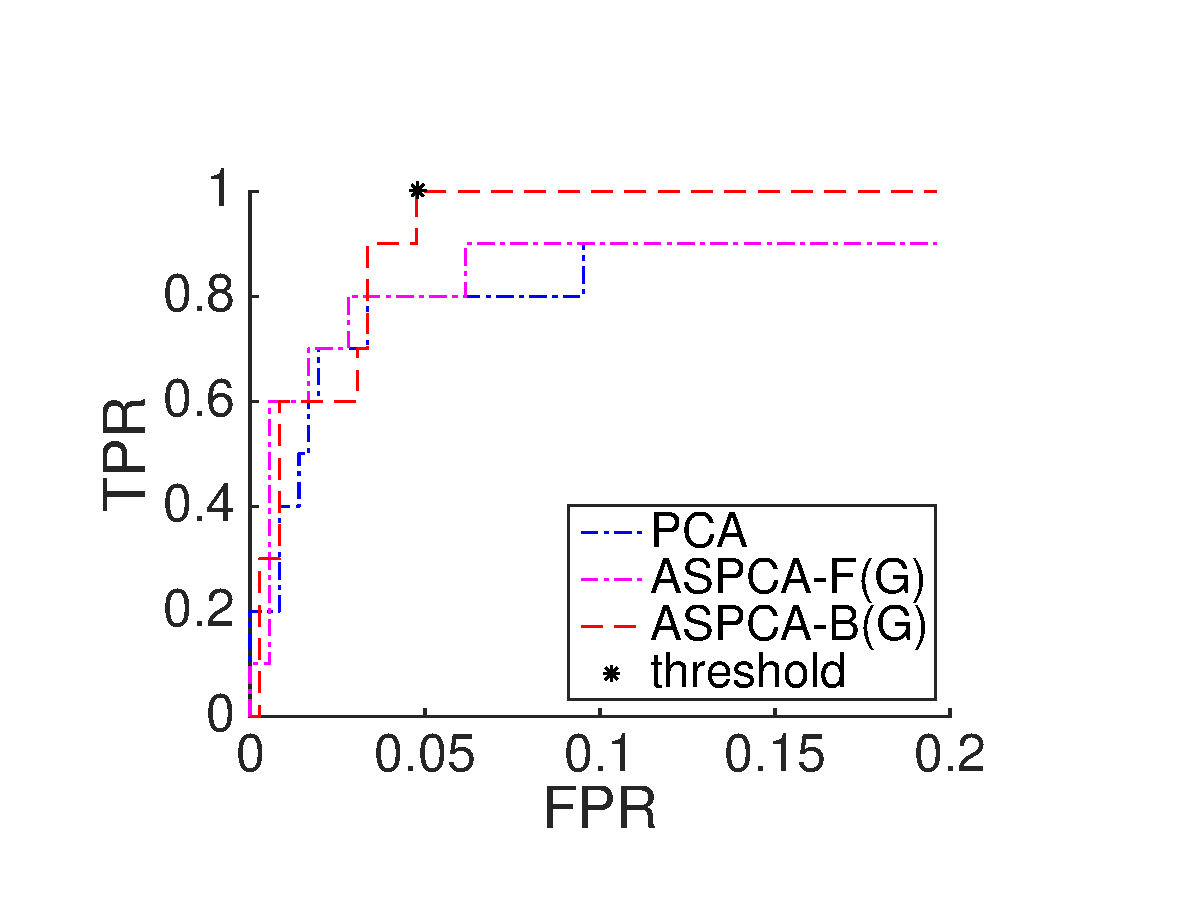
\includegraphics[width=40mm]{figure/new/Cancer-AUC-5}}
    \subcaptionbox{KDD99\label{fig:kdd99:roc}}[3cm] 
  {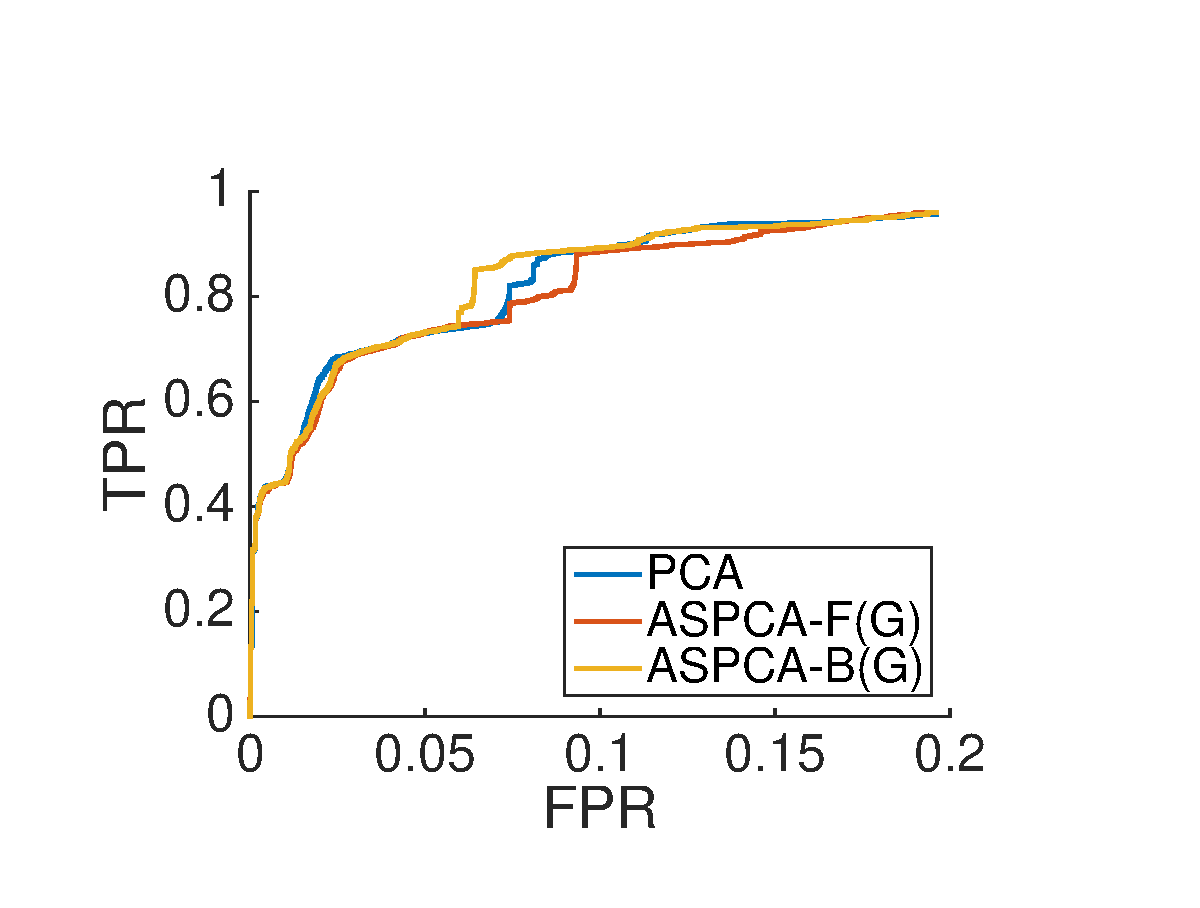
\includegraphics[width=40mm]{figure/new/KDD-AUC-100}}
\caption{ROC curves}
\label{fig:detection performane}
\end{figure}

\subsubsection{稀疏性}
The next set of experiments were designed to compare the sparsity of the loading matrix generated by various ASPCA models and we used the result of PCA as our baseline.  We used three metrics to evaluate the sparsity of the loading matrix of the abnormal PCs, namely,  $||V||_{1,1}$, $Card_{0.1}$ (number of entries with absolute values bigger than 0.1), and $Card_{0.01}$ (number of entries with absolute values bigger than 0.01), and showed the results in Table~\ref{table:sparsity}. We can see that all ASPCA models improved the sparsity of the loading matrix greatly over the baseline. For all datasets, the ASPCA-B model achieved better sparsity performance than the ASPCA-F model. The global optimization step improved $||V||_{1,1}$ values for both models on Breast-Cancer and KDD99. However, in terms of cardinality, ASPCA-FG performed worse than ASPCA-F on Breast-Cancer. The global optimization step achieved the largest sparsity improvement on KDD99, as it has more abnormal PCs than the other two datasets leaving more room for the global optimization. Overall, the ASPCA-BG model achieved the best sparsity performance.

The loading matrices returned by PCA and ASPCA-B (the other three ASPCA models have very similar results) on the Synthetic data are shown in Figure~\ref{fig:mappingmatrix}, and the loading matrices returned by PCA, ASPCA-F, ASPCA-B, ASPCA-FG, ASPCA-BG on Breast-Cancer and KDD99 are shown in Figure~\ref{fig:components}. We can see that ASPCA-F usually leaves some loading vectors with poor sparsity towards the end, which should be avoided as they are part of abnormal subspace. On the contrary, ASPCA-B leaves the loading vectors not so sparse towards the beginning, which need no interpretation as they belong to the normal subspace.

\begin{table}
\small
\caption{Sparsity on Synthetic data, Breast-Cancer, and KDD99}
\begin{tabular}{|l|l|l|l|l|}
\hline
dataset                        & method   & $||V||_{1,1}$ & $card_{0.1}$ & $card_{0.01}$ \\ \hline
\multirow{5}{*}{Synthetic}     & PCA      & 7.07    & 16        & 24           \\ \cline{2-5}
		                       & ASPCA-F  & 5.54    & 9           & 9           \\ \cline{2-5}
		                       & ASPCA-B  & 5.31    & 8          & 8           \\ \cline{2-5}
		                       & ASPCA-FG & 5.54    & 9           & 9           \\ \cline{2-5}
		                       & ASPCA-BG & 5.31    & 8           & 8           \\ \hline
\multirow{5}{*}{Breast-Cancer} & PCA      & 34.22    & 111        & 237           \\ \cline{2-5}
		                       & ASPCA-F  & 17.23    & 33           & 50           \\ \cline{2-5}
		                       & ASPCA-B  & 12.31    & 18          & 18           \\ \cline{2-5}
		                       & ASPCA-FG & 16.50    & 36           & 63           \\ \cline{2-5}
		                       & ASPCA-BG & 12.31    & 18           & 18           \\ \hline
\multirow{5}{*}{KDD99}        & PCA      & 97.33    & 248          & 691           \\ \cline{2-5}
                               & ASPCA-F  & 55.01    & 96           & 265           \\ \cline{2-5}
                               & ASPCA-B  & 54.52    & 101          & 215           \\ \cline{2-5}
                               & ASPCA-FG & 42.77    & 58           & 159           \\ \cline{2-5}
                               & ASPCA-BG & 43.05    & 57           & 157           \\ \hline
\end{tabular}
\label{table:sparsity}
\end{table}

\begin{figure*}
	\centering
    \subcaptionbox{}{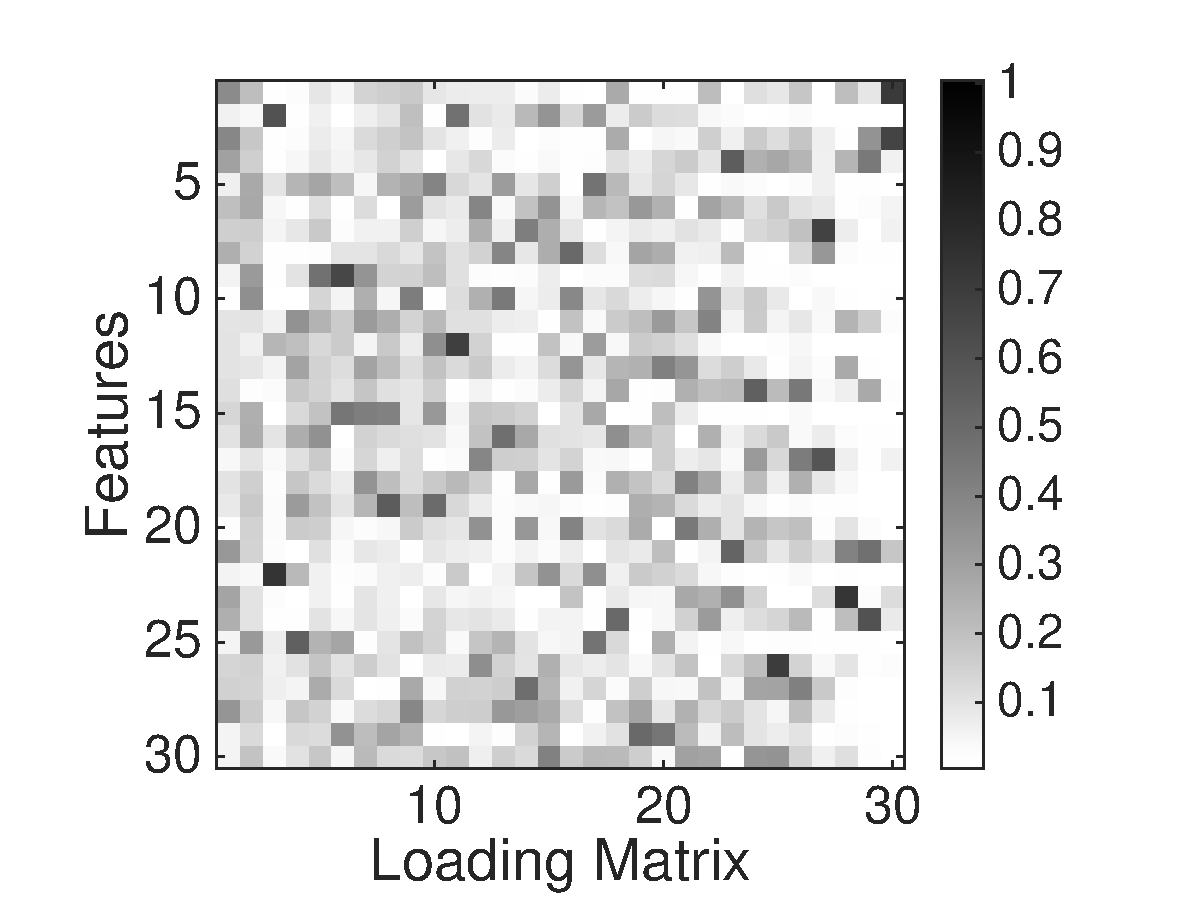
\includegraphics[width=35mm]{figure/new/Cancer-Components-PCA}}
    \subcaptionbox{}{\includegraphics[width=35mm]{figure/new/Cancer-Components-ASPCA-F}}
    \subcaptionbox{}{\includegraphics[width=35mm]{figure/new/Cancer-Components-ASPCA-B}}
    \subcaptionbox{}{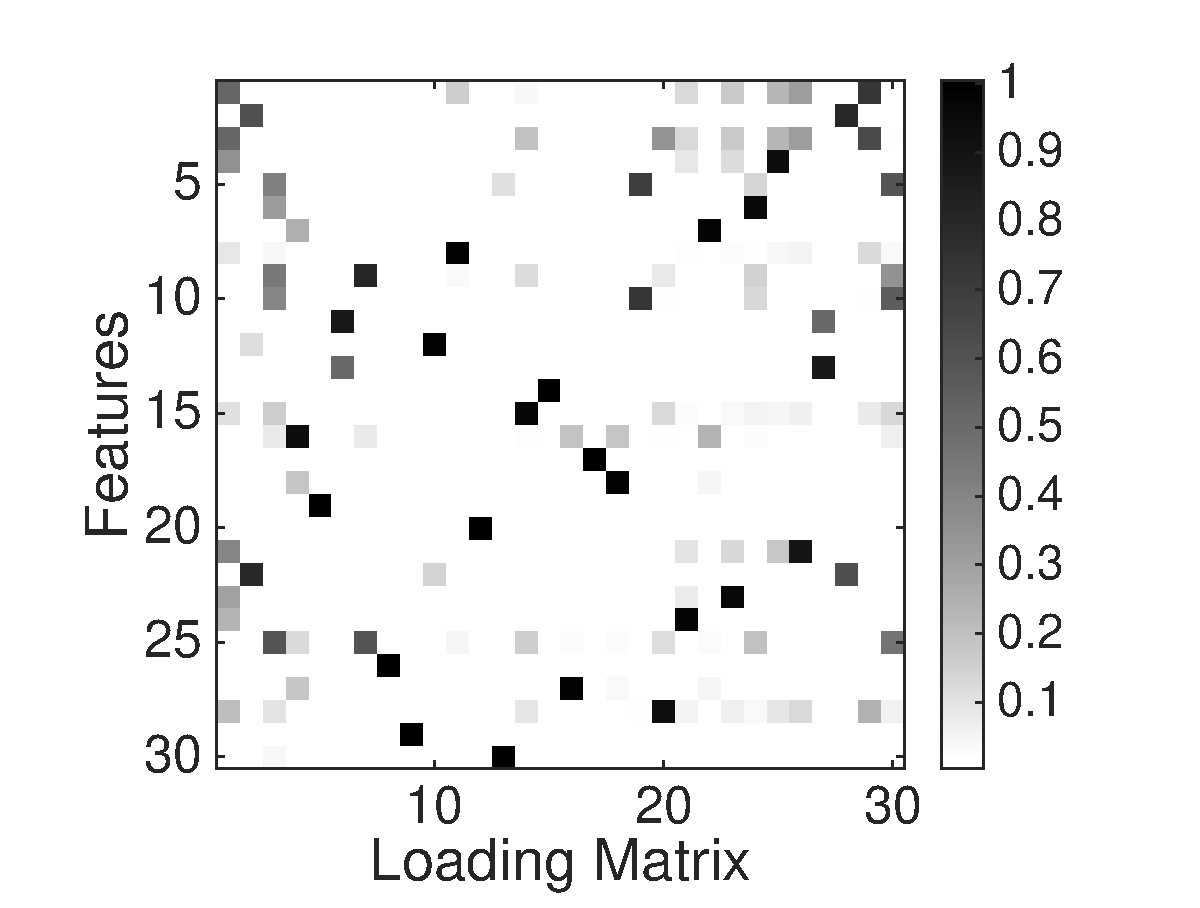
\includegraphics[width=35mm]{figure/new/Cancer-Components-ASPCA-FG}}
    \subcaptionbox{}{\includegraphics[width=35mm]{figure/new/Cancer-Components-ASPCA-BG}}
	\\
    \subcaptionbox{}{\includegraphics[width=35mm]{figure/new/KDD-Components-100-6-PCA}}
    \subcaptionbox{}{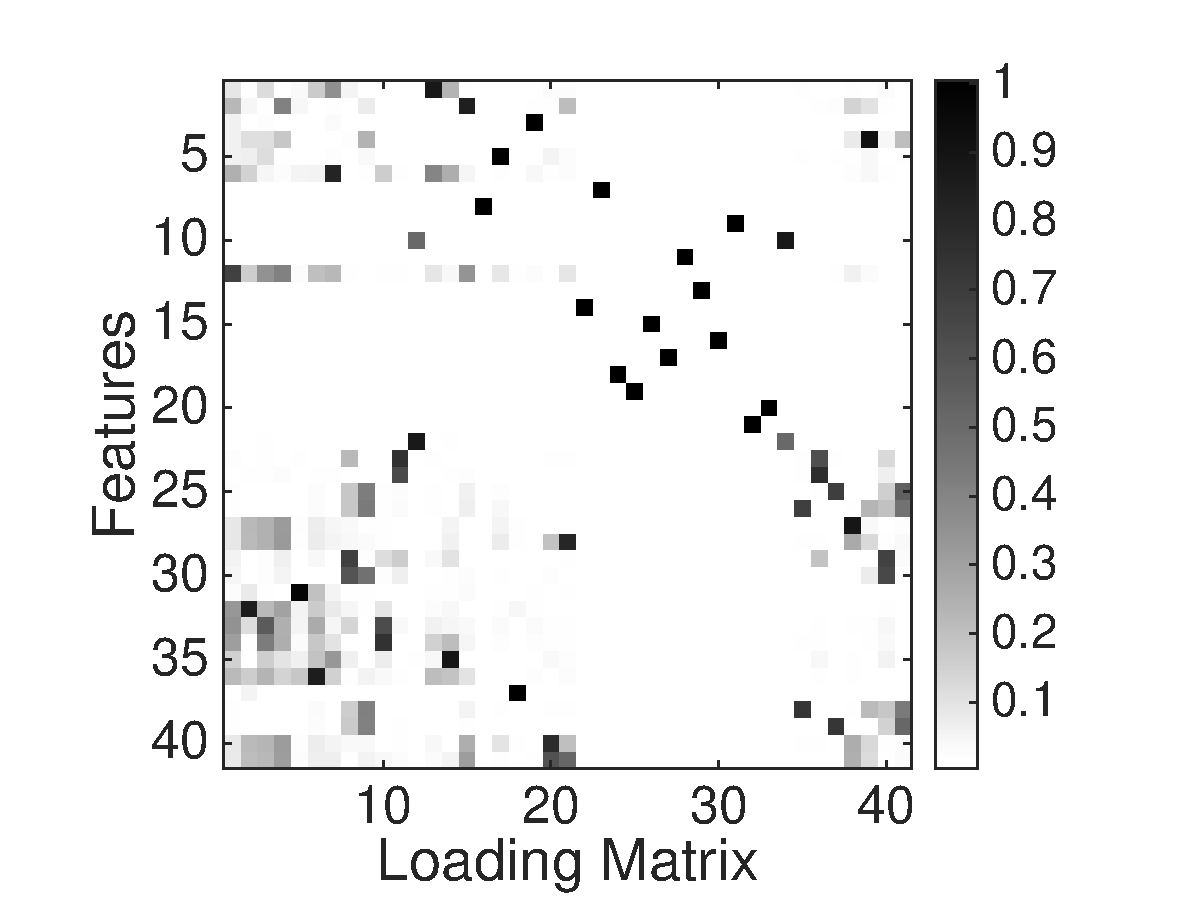
\includegraphics[width=35mm]{figure/new/KDD-Components-100-6-ASPCA-F}}
    \subcaptionbox{}{\includegraphics[width=35mm]{figure/new/KDD-Components-100-6-ASPCA-B}}
    \subcaptionbox{}{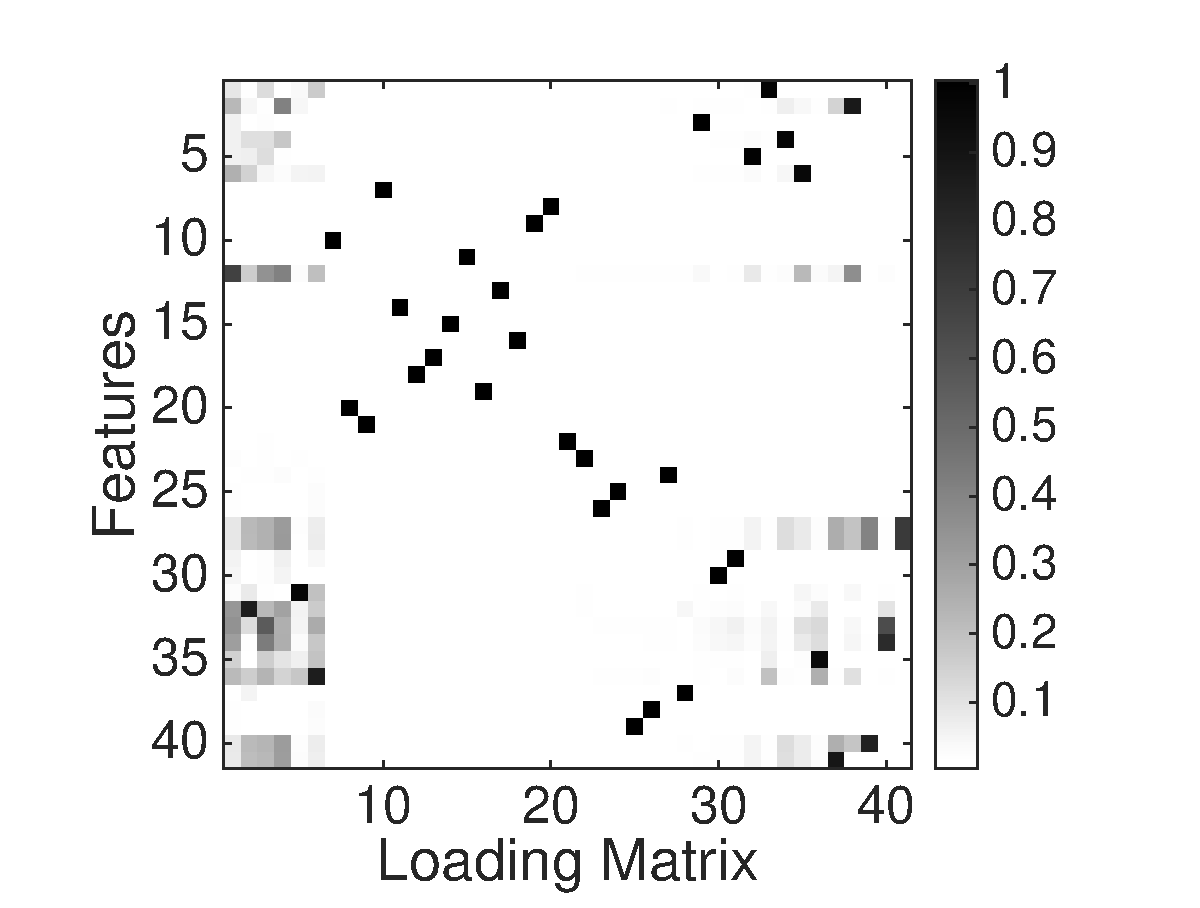
\includegraphics[width=35mm]{figure/new/KDD-Components-100-6-ASPCA-FG}}
    \subcaptionbox{}{\includegraphics[width=35mm]{figure/new/KDD-Components-100-6-ASPCA-BG}}
\caption{Loading matrix of PCs of Breast-Cancer (Top) and KDD99 (Bottom) obtained by PCA, ASPCA-F, ASPCA-B, ASPCA-FG, and ASPCA-BG from left to right}
\label{fig:components}
\end{figure*}

\subsubsection{可解释性}

Now we evaluate the interpretation performance of the ASPCA-BG model, as it has the best sparsity performance. Since we want to see how true anomalies are interpreted by our model, we selected a threshold value on SPE to ensure most of the true anomalies are detected. We show the threshold values, false positive rates (FPR), and true positive rates (TPR) for all three datasets in Table~\ref{table:threshold}.

\begin{table}
\small
\centering
\caption{SPE Threshold}
\begin{tabular}{|l|l|l|l|}
\hline
              & SPE threshold & TPR    & FPR    \\ \hline
Synthetic     & 0.25          & 1      & 0      \\ \hline
Breast-Cancer & 0.1003  & 1      & 0.0476 \\ \hline
KDD99        & 0.5075      & 0.8516 & 0.0657 \\ \hline
\end{tabular}
\label{table:threshold}
\end{table}

{\bf Synthetic Data:}
The four abnormal PCs and the projection values of 15 anomalies on these PCs are shown in Table~\ref{table:components:synthetic} and Figure~\ref{fig:heatmap:synthetic}, respectively. As shown in Table~\ref{table:components:synthetic}, the first three PCs correspond to the rules of $D \approx C + A$, $A \approx B$,  and $F \approx 0$, respectively. The anomalies breaking these rules indeed have large projection values on the corresponding PCs. Thus, our ASPCA-BG model can not only identify the set of
features that are responsible for an anomaly, but also tell the cause of the anomaly, \i.e., breaking the rules indicated by the abnormal PCs.

JSPCA also successfully identified the relevant features $(A, B, D, F)$ as suggested in Figure~\ref{fig:loading matrix:synthetic}. However, it cannot tell the source of each individual anomaly. Unlike JSPCA, our ASPCA models make no assumptions on whether there are anomalies present in the dataset for model training. Keeping only normal data from the Synthetic dataset,  the ASPCA-BG model found four abnormal PCs with loading vectors $(0.31, 0.31, 0.64, 0.64, 0, 0, 0)^T$, $(-0.71,$  $0.71, 0, 0, 0, 0)^T$, $(0, 0, 0, 0, 0, 1, 0)^T$ , and $(0, 0, 0, 0, 0, 0, 1)^T$, which are very similar to the ones in Table~\ref{table:components:synthetic}. Using these abnormal PCs, we can successfully detect and interpret anomalies as well.

\begin{figure}
\centering
	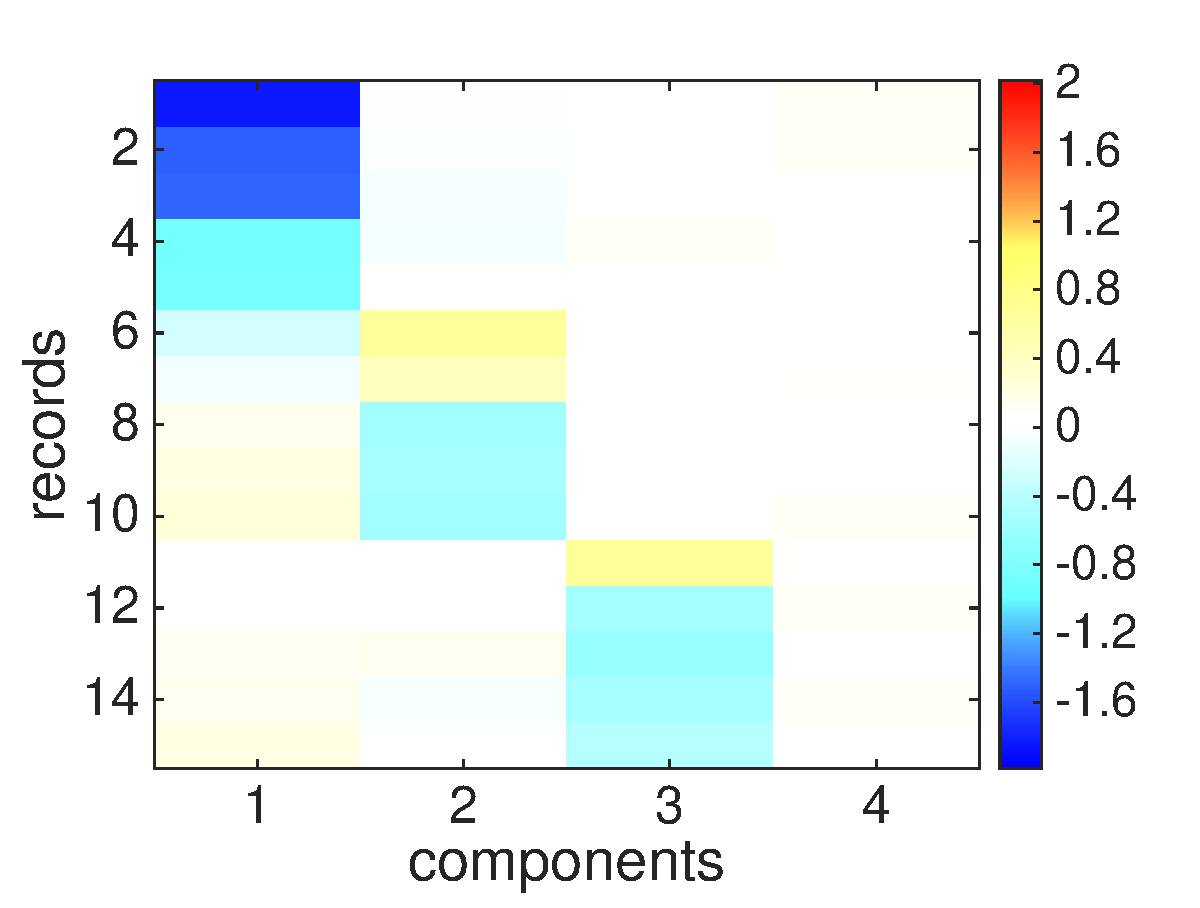
\includegraphics[width=42mm]{figure/new/Synthetic-heat-map}
\caption{Heatmap of projection values of anomalies on abnormal PCs for Synthetic Data}
\label{fig:heatmap:synthetic}
\end{figure}

\begin{table}
\centering
\caption{Components on Synthetic Data}
\label{table:components:synthetic}
\small
\begin{tabular}{|c|c|}
\hline
Index & Components \\ \hline
1 & 0.3099 A + 0.3122 B + 0.6370 C - 0.6330 D \\
2 & 0.7095 A - 0.7047 B\\
3 & 1 F\\
4 & 1 G\\
\hline
\end{tabular}
\end{table}

\begin{figure}
	\centering
	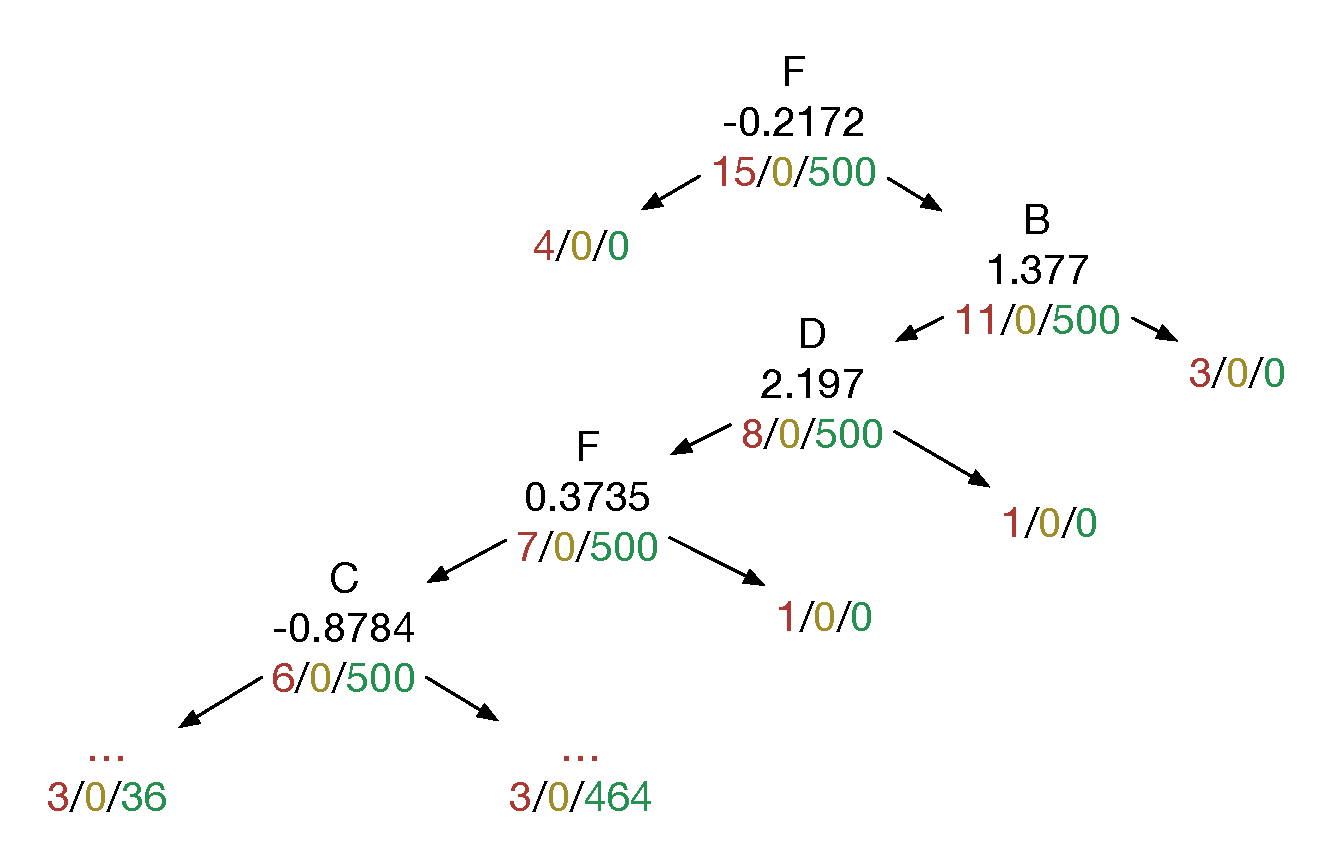
\includegraphics[width=60mm]{figure/new/Synthetic-DT}
	\caption{Decision tree on Synthetic Data}
\label{fig:dt:synthetic}
\end{figure}

The decision tree was shown in Figure~\ref{fig:dt:synthetic}, where on each node we showed the feature and its value used to partition the data, the number of true positives detected by ASPCA-BG in red, the number of false positives in yellow, and the number of normal data detected by ASPCA-BG in green. We can see that the decision tree model needs several rules to describe a group of anomalies which could be easily described by a clear linear combination and a threshold. In Figure~\ref{fig:dt:synthetic}, only the third type of anomalies, which has a large absolute value on F, is easy for the decision tree model to interpret.

{\bf Breast-Cancer:}
The projection values of 10 anomalies on the abnormal PCs obtained by ASPCA-BG for Breast-Cancer are shown in Figure~\ref{fig:heatmap:cancer}.  We can see that the malignant records have two patterns: the first four records have large projection values on the 2nd, 3rd, and 4th PCs, the rest records have large projection values on the first PC and moderate projection values on the 6th PC. We show these PCs in Table~\ref{table:breast_cancer}, where coefficients in PCs less than 0.1 were omitted.  The features appearing in the 1st and 6th PCs are \emph{area\_se}, \emph{area\_worst}, and \emph{radius\_worst}, which were reported previously by \cite{Wolberg1995792} as being effective for classifying malignant records.  Note that, \emph{area\_worst} actually has a quadratic relation with \emph{radius\_worst}, our model identified it as a linear relation, which is a good approximation in a small range of radius. The first four records, on the other hand, do not have large projection values on PCs related to \emph{area} features.  They were detected by PCs related to \emph{symmetry}, \emph{fractal dimension}, and \emph{compactness} features, which clearly indicates another type of malignant records.

\begin{figure}
\centering
	\includegraphics[width=50mm]{figure/new/Cancer-heat-map}
\caption{Heatmap of projection values of anomalies on abnormal PCs of Breast-Cancer}
\label{fig:heatmap:cancer}
\end{figure}

\begin{table}
\caption{Components on Breast-Cancer.}
\label{table:breast_cancer}
\small
\centering
\begin{tabular}{|c|c|}
\hline
Index & Components                                                                                                  \\ \hline
1     & 1 \emph{area\_se}                                                                                       \\ \hline
2     & 0.9894 \emph{symmetry\_worst}             \\ \hline
3     & \begin{tabular}[c]{@{}c@{}}0.9631 \emph{fractal\_dimension\_worst} \\ - 0.2693 \emph{fractal\_dimension\_mean}\end{tabular}                                                                                                 \\ \hline
4     & \begin{tabular}[c]{@{}c@{}}0.9445 \emph{compactness\_worst}\\  - 0.3286 \emph{compactness\_mean}\end{tabular}                                                                                              \\ \hline
%5     &  0.8631 perimeter\_worst - 0.5051 perimeter\_mean\\ \hline
6     & 0.8554 \emph{area\_worst} - 0.5180 \emph{radius\_worst}                                                                                \\ \hline
%7    & 0.8195 area\_mean - 0.5732 radius\_mean                                                                     \\ \hline
%8     & 0.8643 perimeter\_se - 0.5030 radius\_se                                                                    \\ \hline
%9     &     1 concavity\_se                                                        \\ \hline
%10     &    0.9841 fractal dimension\_se                                                                 \\ \hline
\end{tabular}
\end{table}

\begin{figure}
\centering
	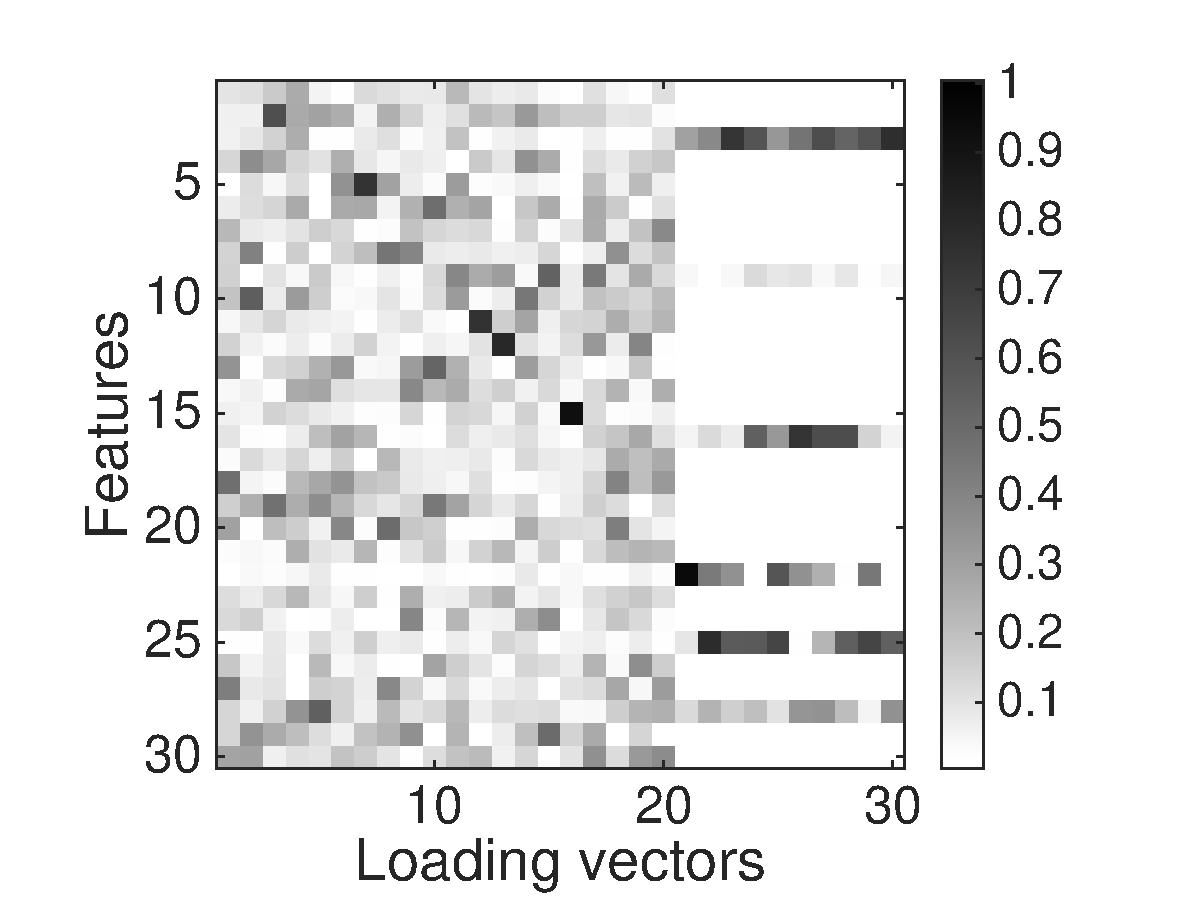
\includegraphics[width=42mm]{figure/Cancer-JSPCA-Components}
\caption{Loading matrix of abnormal PCs obtained by JSPCA on Breast-Cancer}
\label{fig:JSPCA:cancer}
\end{figure}

\begin{figure}
\centering
	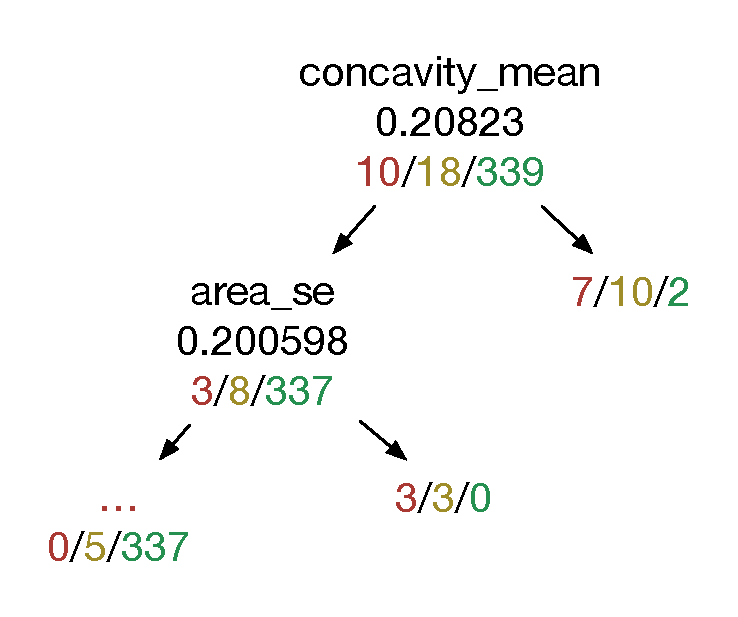
\includegraphics[width=40mm]{figure/new/Cancer-DT}
	\caption{Decision tree on Breast-Cancer}
         \label{fig:tree:cancer}
\end{figure}

The loading matrix of the abnormal PCs obtained by JSPCA on Breast-Cancer is shown in Figure~\ref{fig:JSPCA:cancer}. The relevent features are \emph{radius\_mean}, \emph{concavity\_mean}, \emph{area\_se}, \emph{fractal\_} \emph{dimension\_se}, \emph{perimeter\_worst}, and \emph{compactness\_worst}. As we can see, JSPCA cannot tell the different causes of individual anomalies.
The decision tree obtained on Breast-Cancer is shown in Figure~\ref{fig:tree:cancer}. Our ASPCA-BG model detected 10 true positives, 18 false positives, and 339 true negatives (shown on the root node in red, yellow, and green, respectively) with the chosen SPE threshold. The tree used \emph{concavity\_mean} to separate positive and negative samples. However, the attribute \emph{concavity\_mean} is orthogonal to the abnormal subspace obtained by our ASPCA-BG model, which means it is not the feature based on which our ASPCA-BG model detects anomalies. Hence, using decision trees to interpret results of a subspace-based model, such as ours, may lead to misleading interpretations.

{\bf KDD99:}
With the given SPE threshold, our ASPCA-BG model detected 4397 true positives on KDD99. Although our model is intended to analyze individual anomalies, we can also summarize interpretations of similar anomalies to make our discussion easier. We used a simple way to generate signatures on whether an anomaly has \emph{low} ($\leq -\sqrt{SPE threshold/2}$), or \emph{high} ($\geq \sqrt{SPE threshold/2}$) projection values on the set of abnormal PCs. Then anomalies were grouped according to their signatures, so that the components in the signature of each group is common for most of the anomalies in the group.

In Table~\ref{table:signatures on KDD}, we listed some major signatures found by the above method. Actually, for most of the cases, we can associate each signature group with an anomaly type quite well.  The two numbers listed for each anomaly type are the number of detected anomalies by our model and the number of total anomalies of this type, respectively. The two numbers listed for each signature group are the number of the anomalies of this type and the total number of anomalies in the group, respectively. Some anomaly types only have one main corresponding signature groups, whereas we identified three main signature groups for warezclient{[}R2L{]}. For the $i$th PC, $i$L and $i$H represent low and high projection values on it, respectively.  Finally, the components appeared in these signatures are shown in Table~\ref{table:components on KDD}.

\begin{table}
\small
\caption{Signatures on KDD99}
\label{table:signatures on KDD}
\centering
\begin{tabular}{|c|c|l|}
\hline
                                                                                         & \# in Type/              & Important       \\
Type                                                                                     & \# in Group              & Components      \\ \hline
\multirow{2}{*}{\begin{tabular}[c]{@{}c@{}}neptune{[}DoS{]}\\ 500/500\end{tabular}}      & \multirow{2}{*}{481/484} & 2L, 9H, 10H     \\
                                                                                         &                          & 11H, 12H, 14H   \\ \hline
\begin{tabular}[c]{@{}c@{}}smurf{[}DoS{]}\\ 493/500\end{tabular}                         & 472/472                  & 1H, 3L, 8H, 16H \\ \hline
\begin{tabular}[c]{@{}c@{}}teardrop{[}DoS{]}\\ 496/500\end{tabular}                      & 393/393                  & 18H             \\ \hline
\begin{tabular}[c]{@{}c@{}}satan{[}Probe{]}\\ 500/500\end{tabular}                       & 444/444                  & 2L, 3H, 6H, 8H  \\ \hline
\begin{tabular}[c]{@{}c@{}}portsweep{[}Probe{]}\\ 354/500\end{tabular}                  & 175/175                  & 6H, 7L          \\ \hline
\begin{tabular}[c]{@{}c@{}}ipsweep{[}Probe{]}\\ 217/500\end{tabular}                     & 104/109                  & 1H, 19H         \\ \hline
\multirow{3}{*}{\begin{tabular}[c]{@{}c@{}}warezclient{[}R2L{]}\\ 974/1020\end{tabular}} & 272/395                  & 15H, 20H        \\ \cline{2-3}
                                                                                         & 332/339                  & 4L, 5H, 6L      \\ \cline{2-3}
                                                                                         & 237/292                  & 4L, 5H          \\ \hline
\begin{tabular}[c]{@{}c@{}}guess-passwd{[}R2L{]}\\ 53/53\end{tabular}                    & 48/121                   & 4H, 5H          \\ \hline
\begin{tabular}[c]{@{}c@{}}buffer-overflow{[}U2R{]}\\ 30/30\end{tabular}                 & 7/7                      & 5H, 24H         \\ \hline
\end{tabular}
\end{table}

From Table~\ref{table:signatures on KDD}, we can see that the signatures for different anomaly types varied a lot, from which we often can find the components that are consistent with the nature of each anomaly type. For example, smurf[DoS] attacks are also known as popular form of DoS packet floods, which turn out to have high \emph{srv\_count} and \emph{count} values ({\it i.e.}, 16H and 8H). Teardrop[DoS] attacks try to break the host by sending mangled IP fragments, which led to high \emph{wrong\_fragment} values ({\it i.e.}, 18H).  We can see similar trends for Probe attacks too. For example, ipsweep[Probe] attacks sweep different hosts (IPs) to find cracks for hacking ({\it i.e.}, 19H), whereas portsweep[Probe] attacks try to visit different service ({\it i.e.}, 6H) and short connection duration ({\it i.e.}, 7L). Buffer overflow[U2R] attackers try to gain the root authority on the host, and 24H indicates that the user has logged into the server with root shell. Warezclient[R2L] attackers try to download files in forbidden directories from the FTP servers. Our interpretation is consistent with \cite{sabhnani2003kdd} as \emph{logged\_in} with low \emph{dst\_bytes} ({\it i.e.}, 4L), \emph{is\_guest\_login} ({\it i.e.}, 15H) and high \emph{hot} values ({\it i.e.}, 20H).

\begin{table}
\small
\caption{Components on KDD99}
\label{table:components on KDD}
\centering
	\begin{tabular}{|c|c|}
\hline
Index & Components                                                                                                                   \\ \hline
1     & 0.8906 \emph{protocol\_type} + 0.3658 \emph{logged\_in}                                                                                    \\ \hline
2     & 0.9949 \emph{same\_srv\_rate}                                                                                                       \\ \hline
3     & 0.9958 \emph{diff\_srv\_rate}                                                                                                       \\ \hline
4     & \begin{tabular}[c]{@{}c@{}}0.9520 \emph{dst\_bytes} \\ - 0.2222 \emph{logged\_in}\end{tabular}                                             \\ \hline
5     & \begin{tabular}[c]{@{}c@{}}0.7722 \emph{dst\_host\_same\_srv\_rate} \\ - 0.6286 \emph{dst\_host\_srv\_count}\end{tabular}                  \\ \hline
6     & \begin{tabular}[c]{@{}c@{}}0.9466 \emph{dst\_host\_diff\_srv\_rate}\end{tabular}       \\ \hline
7     & 0.9714 \emph{duration}                                                                                                              \\ \hline
8     & 0.9995 \emph{count}                                                                                                                 \\ \hline
9     & 0.9716 \emph{flag}                                                                                                                  \\ \hline
10    & 0.9984 \emph{dst\_host\_serror\_rate}                                                                                               \\ \hline
11    & 0.9981 \emph{srv\_serror\_rate}                                                                                                     \\ \hline
12    & 0.9981 \emph{serror\_rate}                                                                                                          \\ \hline
14    & 0.9985 \emph{dst\_host\_srv\_serror\_rate}                                                                                          \\ \hline
15    & 0.9997 \emph{is\_guest\_login}                                                                                                      \\ \hline
16    & 0.9994 \emph{srv\_count}                                                                                                            \\ \hline
18    & 0.9996 \emph{wrong\_fragment}                                                                                                       \\ \hline
19    & 0.9970 \emph{dst\_host\_srv\_diff\_host\_rate}                                                                                      \\ \hline
20    & 0.9999 \emph{hot}                                                                                                                   \\ \hline
24    & 1 \emph{root\_shell}                                                                                                                \\ \hline
	\end{tabular}
\end{table}


The results obtained by JSPCA are shown in Table~\ref{Table:KDD 99}. The selected features by JSPCA are more general and similar for all categories. Some of the important features for specific attacks are missing too, for instance, \emph{root\_shell} for User-2-Root[U2R] attacks and \emph{hot} and \emph{is\_guest\_login} for R2L attacks as mentioned in \cite{sabhnani2003kdd}.

We show the decision tree obtained on KDD99 in Figure~\ref{fig:tree:KDD}. The features captured by the decision tree are consistent with the components discovered by our ASPCA-BG model to a large extent. For example, low \emph{same\_srv\_rate} was chosen to detect neptune and satan DoS attackers, which is the same as using 2L in our model to detect the same attacks. Similarly, high \emph{protocol\_type} values ({\it i.e.}, using ICMP protocol) was chosen to detect ipsweep and smurf attackers (detected by 1H in our model). Low \emph{dst\_host\_srv\_count} with high \emph{hot} values is an important character of warezclient and guess-passed attacks  (identical to 5H and 20H in our model). An interesting observation on the decision tree in Figure~\ref{fig:tree:KDD} is that a node on the tree will stop splitting as soon as the samples in the node are mostly positive or negative ones. For example, the left child node of the root in Figure~\ref{fig:tree:KDD} stopped splitting with anomalies from different attack types, in which case, our model can provide more information on the differences of the these attack types.
\begin{figure}
\centering
	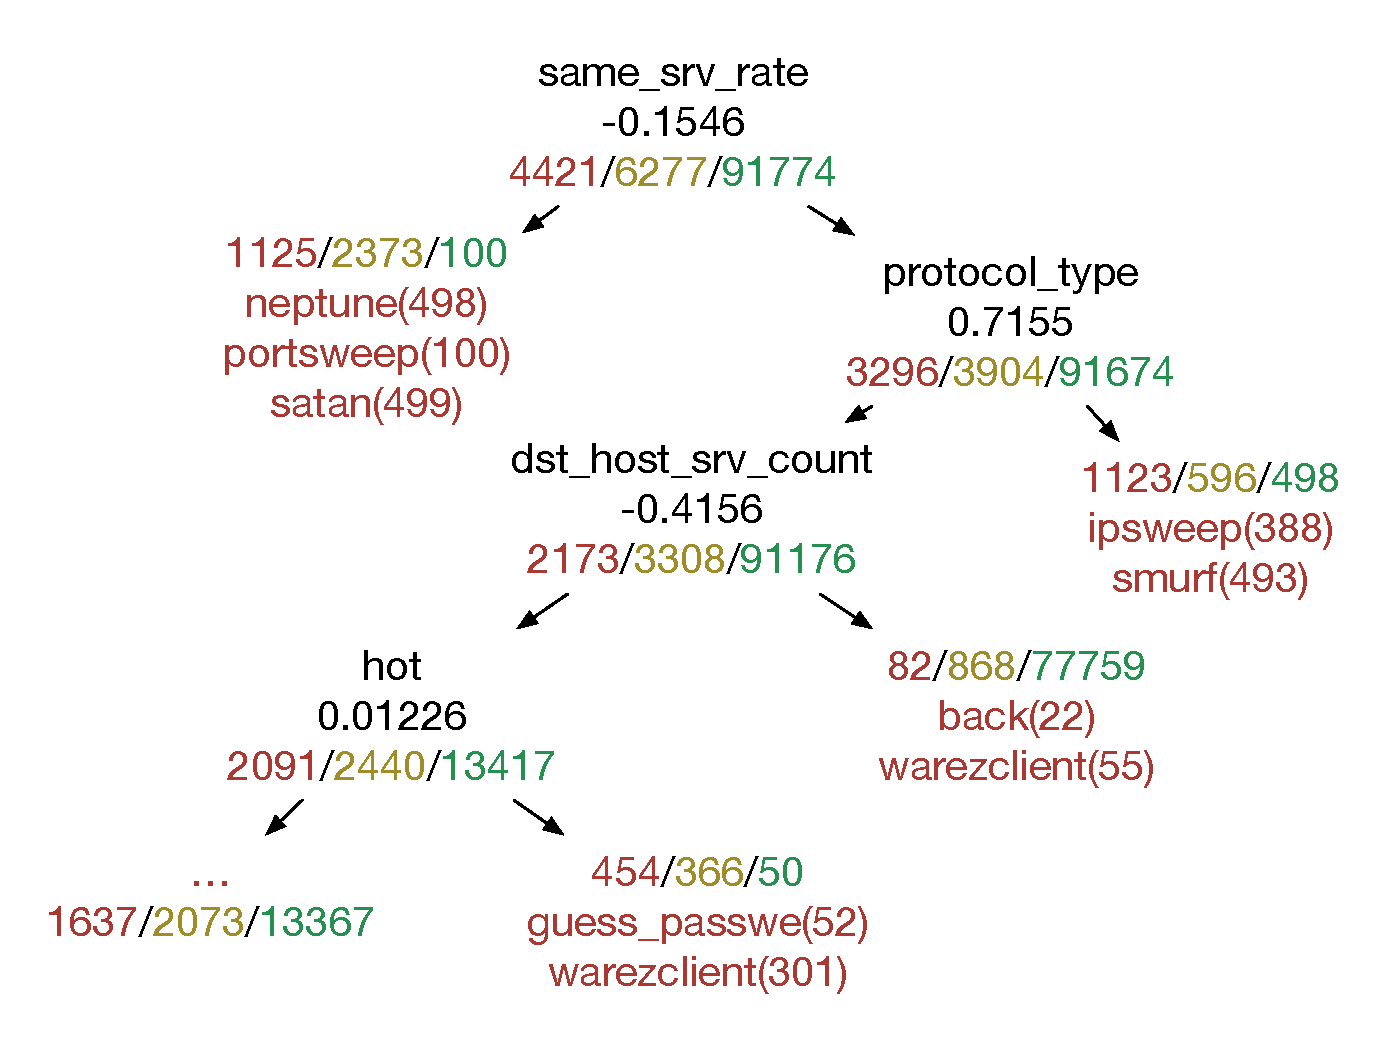
\includegraphics[width=70mm]{figure/new/KDD-DT}
	\caption{Decision tree on KDD99}
         \label{fig:tree:KDD}
\end{figure}


\subsection{Parameter Selection}
\label{sec:parameter}
Our ASPCA models has two parameters to select: the number of abnormal PCs and the coefficient $\lambda$ on sparsity. We know that PCA-based anomaly detection methods are sensitive to the number of PCs \cite{PCA-Sensitivity}. We plotted the detection accuracy (in terms of Area Under ROC Curve (AUC)) with different number of abnormal PCs on Breast-Cancer (with $\lambda=5$) and KDD99 ($\lambda=100$) in Figure~\ref{Figure:parameter:components}. We selected 20 normal PCs ({\it i.e.}, 10 abnormal PCs) for Breast-Cancer data and 6 normal PCs ({\it i.e.}, 35 abnormal PCs), for KDD99 data, to achieve the highest AUC values for our baseline method PCA, to make the comparisons on detection accuracy fair.

The coefficient $\lambda$ is a trade-off between the sparsity and the additional variance on components. With less additional variance, the variances on the whole detection space for various ASPCA models are closer to the one of PCA. We showed the variance, sparsity (valued by $||V||_{1,1}$) and AUC values obtained by varying the value of $\lambda$ on KDD99 and Breast-Cancer in Table~\ref{Table:parameter:lambada} for ASPCA-FG and ASPCA-BG. We can see that our models are not very sensitive to $\lambda$  in terms of AUC, and we selected $\lambda=5$ for Breast-Cancer, $\lambda=100$ for KDD99 for moderate sparsity and variance. The trends are similar for ASPCA-F and ASPCA-B, which were omitted due to space constraints. We selected the same $\lambda$ values for ASPCA-F and ASPCA-B, as in ASPCA-FG and ASPCA-BG, respectively.


\begin{figure}
\centering
\subcaptionbox{Breast-Cancer}
{
	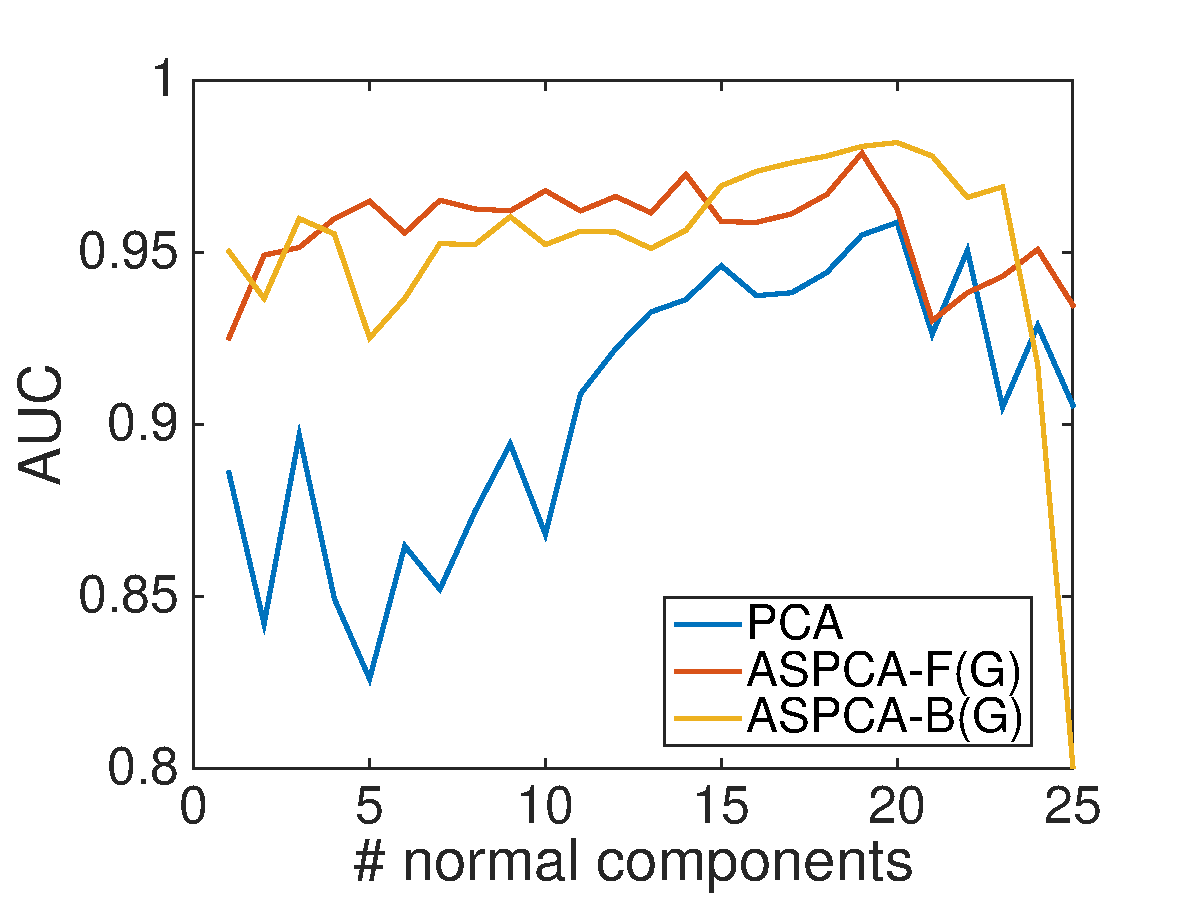
\includegraphics[width=40mm]{figure/new/Cancer-AUC-Components}
}
\subcaptionbox{KDD99}
{
	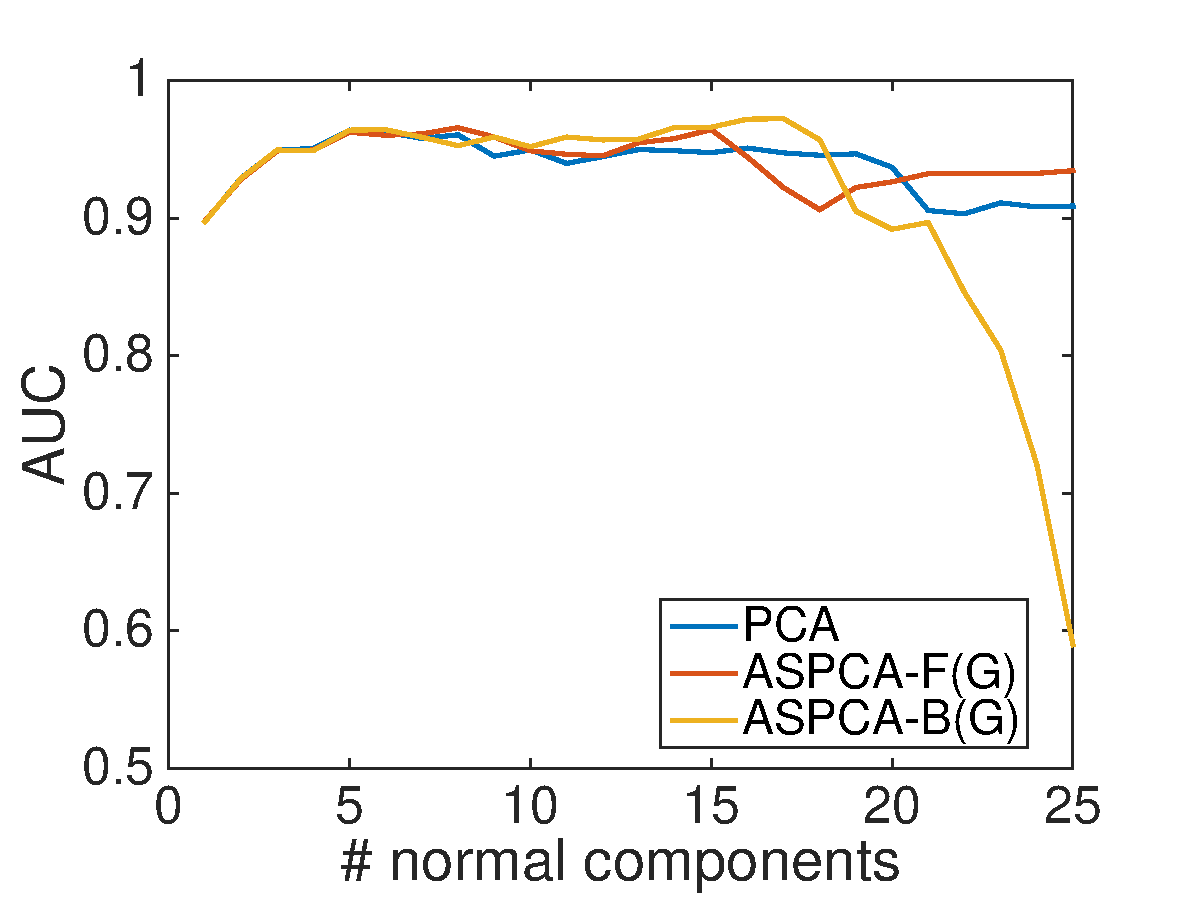
\includegraphics[width=40mm]{figure/new/KDD-AUC-Components}
}
\caption{Selection on the number of normal PCs}
\label{Figure:parameter:components}
\end{figure}


\begin{table*}
\centering
\caption{Selection on $\lambda$ for KDD99}

\begin{tabular}{|l|l|l|l|l|l|l|}
\hline
\multicolumn{1}{|l|}{} & \multicolumn{3}{c|}{ASPCA-FG}    & \multicolumn{3}{c|}{ASPCA-BG}    \\ \hline
$\lambda$ & $||V||_{1,1}$ & Variance & AUC   & $||V||_{1,1}$ & Variance & AUC   \\ \hline
0         & 97.33         & 21518    & 0.963 & 97.33         & 21518    & 0.963 \\
10        & 44.38         & 21524    & 0.963 & 44.59         & 21523    & 0.963 \\
50        & 43.52         & 21627    & 0.962 & 43.97         & 21589    & 0.964 \\
100       & 42.77         & 21873    & 0.960 & 43.04         & 21735    & 0.964 \\
500       & 41.04         & 23673    & 0.956 & 40.67         & 22997    & 0.967 \\ \hline
\end{tabular}
\end{table*}
\begin{table*}
\caption{Selection on $\lambda$ for Breast-Cancer}
\begin{tabular}{|l|l|l|l|l|l|l|}
\hline
\multicolumn{1}{|l|}{} & \multicolumn{3}{c|}{ASPCA-FG}    & \multicolumn{3}{c|}{ASPCA-BG}    \\ \hline
$\lambda$              & $||V||_{1,1}$ & Variance & AUC   & $||V||_{1,1}$ & Variance & AUC   \\ \hline
0                      & 34.23         & 1.2728   & 0.959 & 34.23         & 1.2728   & 0.959 \\
1                      & 26.68         & 14.2012  & 0.903 & 14.95         & 6.2777   & 0.950 \\
5                      & 16.50         & 20.8308  & 0.963 & 12.31         & 20.2968  & 0.982 \\
10                     & 12.81         & 30.8123  & 0.985 & 10            & 57.0009  & 0.966 \\
50                     & 10            & 57.0009  & 0.966 & 10            & 57.0009  & 0.966 \\ \hline
\end{tabular}
	\label{Table:parameter:lambada}

\end{table*}
